\documentclass[12pt]{article}

\usepackage{ediArticle}  %from ediArticle.sty
%\usepackage{multirow}
%\usepackage{amsmath}
%\usepackage[normalem]{ulem}
%\usepackage[table]{xcolor}


%%%%%%%%%%%%%%%%%%%%%%%%%%%%%%%%%%%%%%%%%%%%%%%%%%%%%%
\title{\LARGE \bfseries \vspace{-2cm} Burden and health-related quality of life among caregivers of people with motor neuron disease}
\author{\vspace{-2cm}}
\date{\vspace{-2cm}}

\begin{document}

% Set font size to 13pt
\fontsize{13pt}{15pt}\selectfont

\maketitle


%%%%%%%%%%%%%%%%%%%%%%%%%%%%%%%%%%%%%%%%%%%%%%%%%%%%%%
\section{Introduction}
Motor neuron disease (MND) is a progressive neurodegenerative disease that impacts not only patients but also their informal caregivers. Several studies on ALS in Australia \parencite{lillo_caregiver_2012}, United States \parencite{qutub_life_2014, burke_caregiver_2015, roach_dynamics_2009}, Turkey \parencite{tulek_care_2023}, Ireland \parencite{galvin_caregiving_2016}, Germany \parencite{schischlevskij_informal_2021}, and China \parencite{geng_patients_2017}, have investigated the factors contributing to caregiver burden in ALS and the associated impact of caregiving on the quality of life of these individuals. \textcite{lillo_caregiver_2012} found that patients' abnormal behavior and caregiver stress were the strongest predictors of high caregiver burden, while physical disability was not significantly associated. 

A cross-sectional study of 33 patient-caregiver pairs, which showed that high caregiver burden was associated with greater patient apathy, disinhibition, and executive dysfunction, as well as caregiver distress \parencite{burke_caregiver_2015}. \textcite{qutub_life_2014} study also found that patients' functional status did not affect caregivers' burden. \textcite{schischlevskij_informal_2021} results showed that caregiver burden increased with patients' decline in functional status - patients' wheelchair use and need for supervision were the strongest predictors of burden.

\textcite{tulek_care_2023} study corroborates sex as having a significant relationship to caregivers' burden. \textcite{geng_patients_2017} found an association between caregiver burden and older caregiver age. Other factors related to caregivers' burden are difficulties in managing ALS, the emotional or psychosocial impact of caregiving, limitations or restrictions, and the effects on relationships that caregiving has on the caregivers \parencite{galvin_caregiving_2016}. Patients' functional status affect caregiver quality of life \parencite{roach_dynamics_2009}.

%%%%%%%%%%%%%%%%%%%%%%%%%%%%%%%%%%%%%%%%%%%%%%%%%%%%%%
\section{Methods}

\subsection{Study design and participants}
COMMEND was a XXX designed to YYY. The study design, patient
characteristics, and baseline costs and resource-use data
have been reported \parencite{gould_randomised_2022}. The present study focuses on the caregivers; the baseline characteristics and quality of life have been reported previously for patient  \parencite{gould_acceptance_2024}. Patients with
probable/confirmed?? MND, CRITERIA???, were enrolled between
DATE and DATE, mostly at WHERE. Patients were
also required??? to have a primary caregiver who was
willing to participate in the study. Caregivers were included if BRIEF INCLUSION CRITERIA [cite trial]. 

\subsection{Data and questionnaires}
Data were collected for patients and caregivers at the
baseline visit and at baseline, 6 months, and 18 months during WHICH?? visits. Full details of the baseline patient and caregiver
demographics and characteristics, including comorbidities
and medications used, have been reported previously \parencite{gould_acceptance_2024, keetharuth_costeffectiveness_2024}.

% Paraphrase this
We assessed caregiver burden at every visit using the 22-item version of Zarit Burden Interview (ZBI). ZBI is a widely-used instrument for assessing the perceived burden experienced by caregivers \parencite{zarit_relatives_1980}. The questions cover the caregiver’s health, psychological well-being, finances, social life, and relationship with the patient. The 22-item version of ZBI contains five-point Likert-style questions with responses to each item ranging from 0, denoting “never”, to 4, denoting “nearly always”. \parencite{zarit_hidden_1985}. The total score therefore ranges from 0 to 88, with a higher score indicating a greater perceived care burden. 

% Paraphrase this and shorten
Caregivers self-assessed their HRQoL at using the EuroQol Visual Analogue Scale (EQ-VAS) and 5-dimension (EQ-5D) questionnaires [\textbf{REF}]. For EQ-5D, they scored their current health state in each of five domains (pain/discomfort, anxiety/depression, mobility, usual activities, and self-care) using a 3-point scale (no, moderate, or extreme problems). From the health-state profile obtained, a scoring algorithm using English preference weights [\textbf{REF}] was used to calculate a total utility score (EQ-5D index score) between 0 (represents death) and 1.0 (represents perfect health). Caregivers rated their current health status on the day of assessment using EQ-VAS, which ranges from 0 (worst imaginable health) to 100 (best possible health). The mean norm value in the English population is reportedly XX (\textbf{REF}). 

Factors related to the informal caregivers (\autoref{tab_var_category}), that is age,sex, educational level, work status, change in work status, relation to the patient with ALS, and whether cohabiting with the patient, was collected with the study‐specific questionnaire. It also included questions on time spent on informal caregiving in personal ADL (P‐ADL),that is feeding, bathing, dressing, toileting and transfer; instrumental ADL (I‐ADL), that is cooking, transport, cleaning and shopping; andother activities that the patient with ALS used to do before disease onset. The first set of variables were caregiver sociodemographic characteristics.  such as sex (DEFINE), age (DEFINE), level of education (DEFINE), employment status (DEFINE). We also asked respondents if they had any medical conditions. Other variables were caregiving context, including relationship with care recipient (DEFINE), intensity of caregiving activities (DEFINE), and how long has been looking after (DEFINE).

We also collected information on characteristics of patients with ALS (\autoref{tab_var_category}). These included age, sex, marital status, employment situation, educational level, presence and number of comorbidities, duration of disease, disease severity. These were collected during XXX \parencite{gould_acceptance_2024}. Disease severity was measured using the ALS Functioning Rating Scale‐Revised, ALSFRS‐R \parencite{cedarbaum_alsfrs-r_1999}. We used the algorithm developed by \textcite{balendra_estimating_2014} to calculate King's clinical stages from ALSFRS-R scores. The King's staging system is based on disease burden and consists of five disease stages (1 to 5) with stage 1 being onset of disease in one anatomical region and stage 5 being death.

\hspace{1em}
\begin{table}[H]
    \centering \singlespacing \small
    \caption{Categorization of independent variables}
    \begin{tabular}{|L{6cm}|L{9cm}|}
        \hline
        \PlainInput{tables/tab_var_category}
    \end{tabular}
    \label{tab_var_category}
    \caption*{\footnotesize \textit{Notes:} Donec sit amet viverra justo}
\end{table}


\subsection{Statistical analysis}
We described the characteristics of the participants (patients with MND and caregivers) using means and standard deviations for continuous variables and using numbers and percentages for categorical variables. We used univariate linear regression to examine the direction and size of the relationships between caregiver burden and possible influencing factors on  caregivers’ burden (ZBI) and health-related quality of life (EQ-5D). We then conducted a multiple regression analysis to test the extent to which these variables explained ZBI and EQ-5D. We selected variables to add to multiple linear regression by adopting a critical level of significance (p ≤ 0.10) in the univariate analysis.

All analysis were conducted using Stata version 18.0 (StataCorp, College Station, Texas, USA).

\section{Results}
Descriptive statistics in (\autoref{tab_desc_stat}). 

\hspace{1em}
\begin{table}[H]
    \centering \singlespacing \small
    \caption{Descriptive statistics.}
    \begin{tabular}{|L{5cm}|R{3.2cm}|}
        \hline
        \PlainInput{tables/tab_desc_stat}
    \end{tabular}
    \label{tab_desc_stat}
    \caption*{\footnotesize \textit{Notes:} Data are based on participants with non-missing baseline caregiver burden and quality of life data. n, number; SD, standard deviation.
}
\end{table}



\hspace{1em}
\begin{figure}[H]
    \centering
    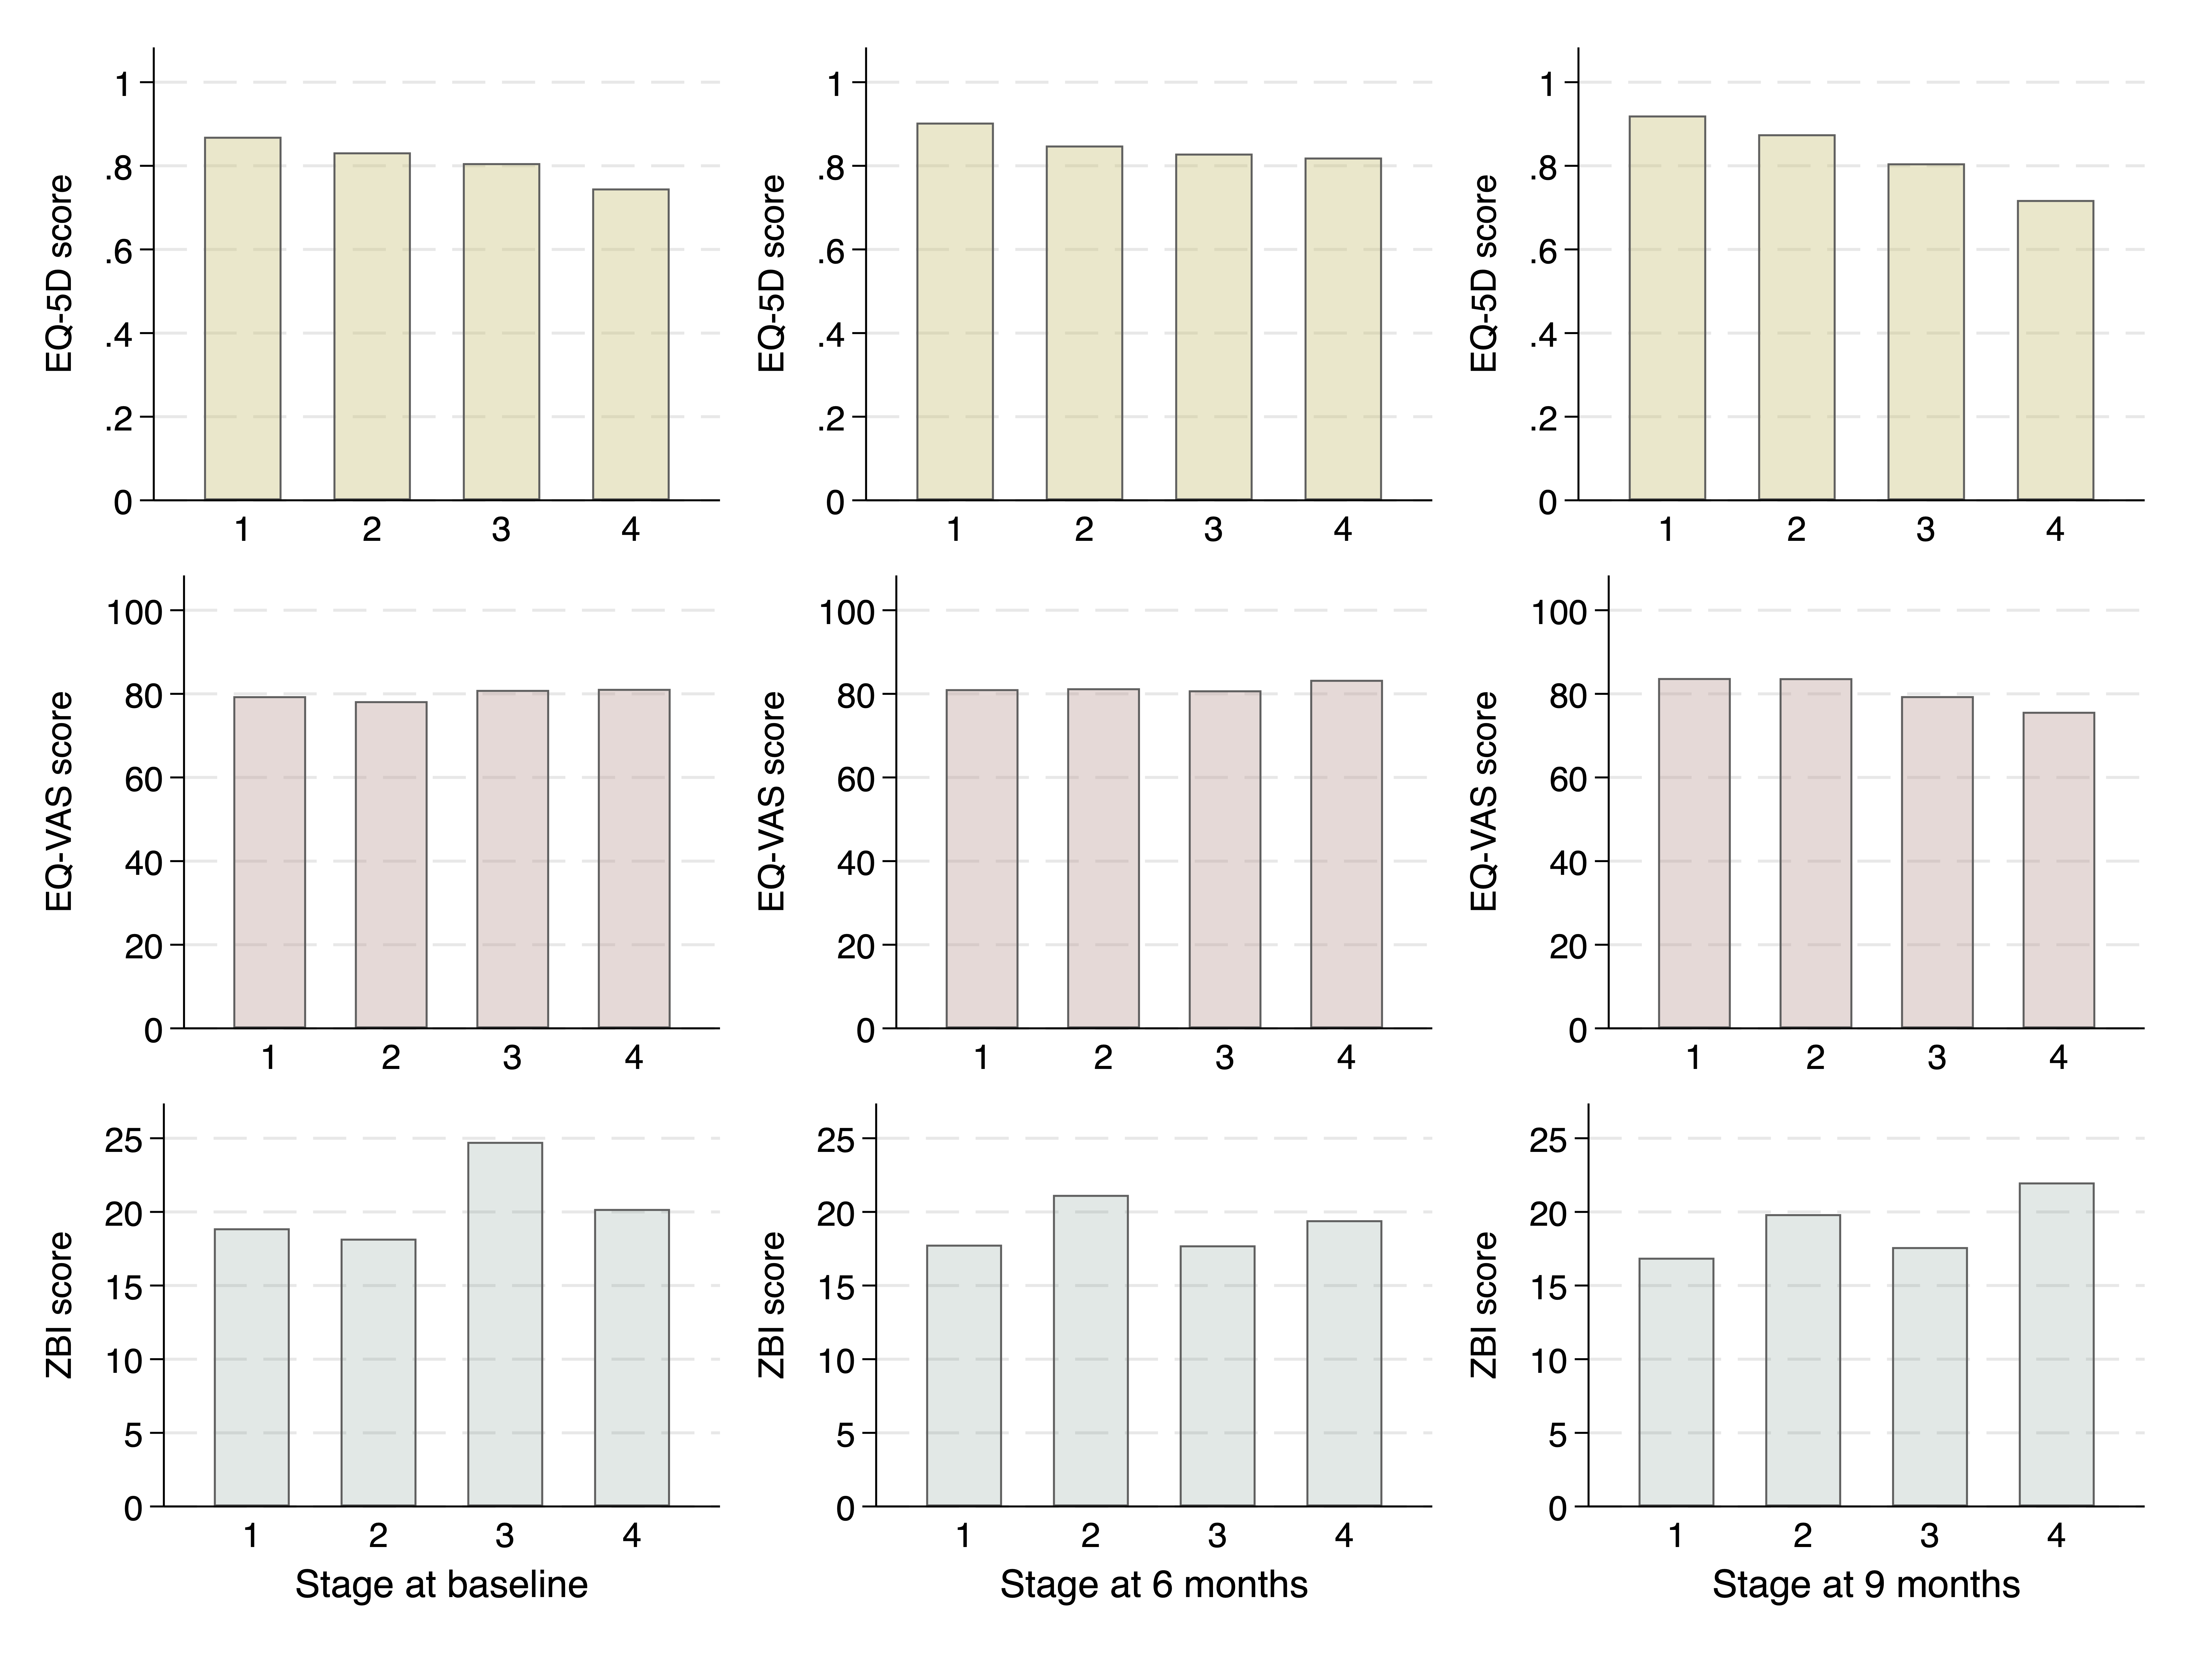
\includegraphics[width=1\linewidth]{figures/outcome-kings-stage.png}
    \caption{EQ-5D-5L utility scores, domain scores and scores by King’s stage}
    \label{fig:outcome-kings-stage}
    \caption*{\footnotesize \textit{Notes:} }
\end{figure}

\hspace{1em}
\begin{table}[H]
    \centering \singlespacing \small
    \caption{Pooled carer ZBI, EQ-VAS, and EQ-5D utility and domain scores by King’s stage}
    \begin{tabular}{|L{.33\linewidth}|R{.1\linewidth}|R{.1\linewidth}|R{.1\linewidth}|R{.1\linewidth}|R{.1\linewidth}|}
        \hline
        \PlainInput{tables/tab_outcomes_kings}
    \end{tabular}
    \label{tab_outcomes_kings}
    \caption*{\footnotesize 
                \textit{Notes:} Data from all caregivers at all time points (baseline, 6 months, and 9 months) have been pooled. Comparisons of outcomes between King’s stages use ANOVA. ZBI total score ranges from 0 to 88, with higher scores indicating greater burden. EQ-5D scores range from 0 to 1.0, with higher scores indicating better health-related quality of life. EQ-VAS scores range from 0 to 100, with higher scores indicate better health-related quality of life. EQ-5D domain scores range from 0 to 3, with higher scores indicating greater restriction by domain. \\
                ANOVA, analysis of variance; EQ-5D, EuroQol 5-dimension questionnaire; VAS, visual analog scale; ZBI, Zarit Burden Interview}
\end{table}



\section{Discussion}
%%%%%%%%%%%%%%%%%%%%%%%%%%%%
%%% %%%
%%% Bibliography %%%

\clearpage
\newrefcontext[sorting=nyt]
\printbibliography


\end{document}
